\documentclass[10pt,twocolumn,letterpaper]{article}

\usepackage[utf8]{inputenc}
\usepackage[margin=0.75in]{geometry}
\usepackage{amsmath,amssymb,amsfonts}
\usepackage{booktabs}
\usepackage{graphicx}
\usepackage{microtype}
\usepackage{cite}
\usepackage{url}
\usepackage{algorithm2e}
\usepackage{listings}
\usepackage{xcolor}
\usepackage{tikz}
\usetikzlibrary{shapes.geometric, arrows.meta, positioning, calc}
\usepackage[colorlinks=true,linkcolor=blue,citecolor=blue,urlcolor=blue]{hyperref}

\definecolor{codegreen}{rgb}{0,0.6,0}
\definecolor{codegray}{rgb}{0.5,0.5,0.5}
\definecolor{codepurple}{rgb}{0.58,0,0.82}
\definecolor{backcolour}{rgb}{0.97,0.97,0.97}

\lstdefinestyle{mystyle}{
    backgroundcolor=\color{backcolour},
    commentstyle=\color{codegreen},
    keywordstyle=\color{magenta},
    numberstyle=\tiny\color{codegray},
    stringstyle=\color{codepurple},
    basicstyle=\ttfamily\footnotesize,
    breakatwhitespace=false,
    breaklines=true,
    captionpos=b,
    keepspaces=true,
    numbers=left,
    numbersep=5pt,
    showspaces=false,
    showstringspaces=false,
    showtabs=false,
    tabsize=2
}
\lstset{style=mystyle}

\title{\textbf{AgentsX: A Resilient, Zero-Overhead, and Sandbox-Hardened Runtime Harness for Autonomous Agents}}

\author{
    \textbf{AgentsX Core Research Team} \\
    \texttt{\{research, engineering\}@agentsx.org}
}

\date{\today}

\begin{document}

\maketitle

\begin{abstract}
Large Language Model (LLM)-driven autonomous agents are fundamentally transforming computational problem solving and human-machine collaboration. However, deploying autonomous agent runtimes on developer or enterprise host systems exposes a persistent architectural \emph{trilemma}: (1) \textbf{Virtualization Overhead vs. Operational Agility}: containerized platforms (e.g., OpenHands, SWE-agent) mandate heavy Docker daemons, introducing multi-second cold-start latency and container-host boundary frictions; (2) \textbf{Black-Box Security vs. Boundary Escape}: commercial terminal tools either demand all-or-nothing command permissions or lack operating-system-level path confinement, leaving host files vulnerable to directory traversal via sub-tool parameters (such as bash working directories); and (3) \textbf{Long-Horizon Thrashing vs. Runaway Token Consumption}: long trajectories suffer from catastrophic token burnout caused by repeated tool invocation loops or fragile context compaction pipelines.

To resolve these challenges, we present \textbf{\textsc{AgentsX}}, an open-source, resilient, zero-overhead, and sandbox-hardened runtime harness for general-purpose autonomous agents. Rather than narrowing scope to a single task, \textsc{AgentsX} provides an extensible agent operating foundation equipped with native Model Context Protocol (MCP) client connectivity, web intelligence retrieval, hierarchical subagent delegation, and multimodal ingestion. We treat complex Software Engineering (Coding/SE) as the flagship stress-testing domain to empirically benchmark the harness under extreme real-world reasoning, state mutation, and execution pressures.

Guided by the design doctrine of \emph{``Effective and Simple,''} \textsc{AgentsX} introduces: (i) a pure asynchronous generator-based, lock-free event-driven ReAct core with $<30\,\text{ms}$ cold start and sub-$50\,\text{MB}$ RSS; (ii) a zero-trust three-tier defensive security sandbox featuring canonicalized path resolution with symlink-traversal tracking (\texttt{PathGuard}), bash Abstract Syntax Tree command filtering (\texttt{CommandGuard}), and human-in-the-loop interactive approval callbacks (\texttt{ApprovalCallback}) that strictly confine file operations and bash working directories without container overhead; (iii) a progressive two-tier circuit-breaker watchdog that injects soft corrective guidance before hard-tripping to eliminate infinite loop thrashing; and (iv) a fault-tolerant dual-stage semantic context compaction engine coupled with semantic single-line micro-pruning that cuts long-horizon token expenditure by up to $65\%$ while maintaining full operational accuracy. Comprehensive empirical evaluations across 510+ regression tests, security penetration vectors, and multi-turn refactoring benchmarks demonstrate that \textsc{AgentsX} achieves enterprise-grade host security, fault-tolerant execution resilience, and superior agility compared to existing closed- and open-source paradigms.
\end{abstract}

\section{Introduction}
\label{sec:intro}

The evolution of Large Language Models (LLMs) from passive text completion engines~\cite{chen2021evaluating} to proactive autonomous agents~\cite{yao2023react, schick2023toolformer} marks a paradigm shift in computing. Modern autonomous agents are expected to act as general-purpose problem-solving runtimes capable of navigating file systems, browsing the live web, dispatching sub-agents, interacting with enterprise APIs, and executing shell commands on host machines.

Despite rapid advancements, deploying autonomous agents into host developer environments has revealed severe architectural contradictions, which we formulate as \textbf{The Trilemma of Autonomous Agent Systems} (Figure~\ref{fig:trilemma}):

\begin{figure}[htbp]
\centering
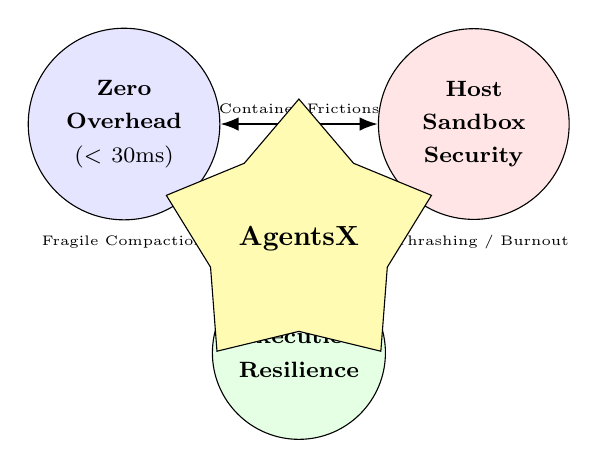
\begin{tikzpicture}[node distance=2.2cm, auto, >=Latex]
    \node [draw, circle, fill=blue!10, text width=1.8cm, text centered] (agile) {\footnotesize \textbf{Zero Overhead} ($<30\text{ms}$)};
    \node [draw, circle, fill=red!10, text width=1.8cm, text centered, right=2.0cm of agile] (secure) {\footnotesize \textbf{Host Sandbox Security}};
    \node [draw, circle, fill=green!10, text width=1.8cm, text centered, below=1.8cm of $(agile)!0.5!(secure)$] (resilient) {\footnotesize \textbf{Execution Resilience}};

    \draw [<->, thick] (agile) -- node [above] {\tiny Container Frictions} (secure);
    \draw [<->, thick] (secure) -- node [right] {\tiny Thrashing / Burnout} (resilient);
    \draw [<->, thick] (resilient) -- node [left] {\tiny Fragile Compaction} (agile);

    \node at ($(agile)!0.5!(secure)!0.5!(resilient)$) [draw, star, star points=5, fill=yellow!30, inner sep=2pt] {\textbf{\textsc{AgentsX}}};
\end{tikzpicture}
\caption{The Trilemma of Autonomous Agent Systems. Existing architectures sacrifice developer agility (OpenHands), fine-grained host security (Claude Code), or execution resilience (experimental prototypes). \textsc{AgentsX} reconciles all three dimensions.}
\label{fig:trilemma}
\end{figure}

\begin{enumerate}
    \item \textbf{Virtualization Overhead vs. Operational Agility}: Heavyweight systems such as OpenHands~\cite{openhands2024} and SWE-agent~\cite{yang2024sweagent} prioritize sandboxing by encapsulating executions inside Docker containers or virtual machines. While containerization provides process isolation, it introduces prohibitive frictions: multi-second cold starts, multi-gigabyte memory footprints, complex volume mounts, and network boundary barriers that break access to local SSH credentials, hardware keys, and local language servers.
    \item \textbf{Black-Box Security vs. Boundary Escape}: Conversely, lightweight terminal agents (e.g., Claude Code~\cite{anthropic2024claudecode} and raw Python scripting harnesses) execute commands directly on the host machine. However, they typically rely either on coarse-grained, all-or-nothing user prompts or naive string prefix checks (e.g., \texttt{path.startswith(workspace)}). Attackers or hallucinating models can bypass these checks via directory traversal (\texttt{../../}), symbolic link dereferencing, or subtle working directory escapes in terminal tools (e.g., invoking \texttt{tool\_bash(cwd="../../sensitive")}).
    \item \textbf{Long-Horizon Thrashing vs. Runaway Token Costs}: In complex multi-turn tasks, models frequently succumb to ``loop thrashing''---repeatedly issuing identical failed tool calls or failing to recover from error traces. Without an active supervisor, agents burn through their token budget until reaching global step cutoffs. Furthermore, naive context compaction frequently truncates vital system instructions, whereas pure LLM-based summarization introduces single-point failure risks during API timeouts or rate limits.
\end{enumerate}

To overcome these fundamental challenges, we present \textbf{\textsc{AgentsX}}, an open-source, production-grade autonomous agent runtime harness engineered under the principle of \emph{``Effective and Simple.''} 

\noindent\textbf{Why Software Engineering as Flagship Benchmark?} We specifically deploy complex Software Engineering (Coding/SE) tasks~\cite{jimenez2024swebench} as our primary stress-testing domain. Software engineering represents the most challenging operational environment for autonomous agents: it demands rigorous multi-step deductive reasoning, involves destructive host mutations (file rewrites and arbitrary shell execution), generates high-volume diagnostic outputs, and induces frequent error states. Demonstrating zero-escape host security, resilience against thrashing, and low-latency agility in software engineering provides definitive validation of \textsc{AgentsX} as a general-purpose agent runtime.

\noindent\textbf{Key System Contributions}:
\begin{itemize}
    \item \textbf{Pure Async Event-Driven Core}: We formulate the ReAct loop as an asynchronous generator yielding strongly typed immutable events. \textsc{AgentsX} eliminates framework lock-in, achieving $<30\,\text{ms}$ initialization latency and $<50\,\text{MB}$ memory footprint.
    \item \textbf{Zero-Trust Three-Tier Security Sandbox}: We propose a deterministic, multi-layer host sandbox comprising canonicalized path resolution with symlink dereferencing (\texttt{PathGuard}), bash Abstract Syntax Tree command validation (\texttt{CommandGuard}), and an interactive Human-in-the-Loop approval callback (\texttt{ApprovalCallback}). We enforce strict workspace confinement across file tools and terminal execution working directories without container overhead.
    \item \textbf{Progressive Two-Tier Circuit-Breaker Watchdog}: We develop a watchdog supervisor that monitors sliding-window tool repetition and error frequencies, injecting soft corrective system prompts at Level 1 before tripping a hard circuit breaker at Level 2, saving over $90\%$ of wasted tokens during model thrashing.
    \item \textbf{Fault-Tolerant Dual-Stage Compaction with Micro-Pruning}: We introduce a robust context compaction pipeline that combines deterministic single-line tool result summarization (\texttt{ToolResultPruner}) with structured three-element LLM semantic compression, guarded by a zero-overhead fallback mechanism and head-tail preserving log truncation.
    \item \textbf{Open Protocol Extensibility and Empirical Validation}: We engineer native integration with the Model Context Protocol (MCP), live web exploration tools, and multimodal input pipelines, validated across 510+ automated tests, security penetration vectors, and long-horizon benchmarks.
\end{itemize}

\section{Comparative Landscape}
\label{sec:related}

To contextualize \textsc{AgentsX}, we categorize state-of-the-art coding agent frameworks into three paradigms and compare them across ten foundational system dimensions in Table~\ref{tab:comparison}:

\begin{table*}[t]
\centering
\small
\caption{Systematic Architectural Comparison Across Leading Autonomous Coding Systems.}
\label{tab:comparison}
\begin{tabular}{lcccccc}
\toprule
\textbf{Architectural Dimension} & \textbf{Claude Code} & \textbf{OpenAI Assist.} & \textbf{OpenHands} & \textbf{DeepSeek-Harness} & \textbf{Pi-Agent} & \textbf{\textsc{AgentsX} (Ours)} \\
\midrule
\textbf{Architecture Paradigm} & Terminal CLI & Managed API & Microservices/Docker & Evaluation Script & Research Prototype & \textbf{Async Embedded Core} \\
\textbf{Open Source Status} & Proprietary & Proprietary & Open Source & Open Source & Open Source & \textbf{Open Source (MIT/Apache)} \\
\textbf{Cold Start Latency} & $\approx 1.2\,\text{s}$ & Network bounded & $4.8\,\text{s} - 15\,\text{s}$ & $\approx 45\,\text{ms}$ & $\approx 35\,\text{ms}$ & $\mathbf{< 30\,\text{ms}}$ \\
\textbf{Runtime Footprint} & Node.js ($\approx 120\text{M}$) & Cloud-hosted & Docker Daemon ($>1\text{G}$) & Minimal Python & Minimal Python & \textbf{Pure Python ($< 50\text{MB}$)} \\
\textbf{Model Portability} & Anthropic only & OpenAI only & LiteLLM Proxy & DeepSeek focused & Single model & \textbf{Multi-Provider Native} \\
\textbf{Sandbox Isolation} & Coarse Prompts & Cloud Sandbox & Docker Containers & Timeout only & Unconstrained & \textbf{Three-Tier Path/AST Guard} \\
\textbf{Bash CWD Escape Guard} & Black-box & Cloud bounded & Container bounded & None & None & \textbf{Strict PathGuard Confinement} \\
\textbf{Loop Thrashing Mitigation} & Model autonomy & Step cutoff & Step limit cutoff & Step limit cutoff & None & \textbf{Two-Tier Progressive Breaker} \\
\textbf{Context Compaction} & Prompt caching & Sliding window & Basic truncation & Raw history & Naive slice & \textbf{Dual-Stage + Micro-Pruning} \\
\textbf{Cache Hit Telemetry} & Internal & Hidden & Basic token count & Token count & None & \textbf{Real-Time Hit-Rate (\texttt{/status})} \\
\textbf{RSI \& Revert Mechanism} & \texttt{CLAUDE.md} rules & None & Session restart & Static bench & Tree branch & \textbf{Crystallization + Tree Revert} \\
\bottomrule
\end{tabular}
\end{table*}

\subsection{Heavyweight Virtualized Platforms}
Frameworks such as OpenHands~\cite{openhands2024} and SWE-agent~\cite{yang2024sweagent} construct an execution harness atop Docker containers. While effective for isolated benchmark evaluation (e.g., SWE-bench~\cite{jimenez2024swebench}), this design introduces high cold-start latency, resource hogging, and isolation from host developer environments, making them unsuited as lightweight command-line companion tools.

\subsection{Proprietary Terminal Agents}
Claude Code~\cite{anthropic2024claudecode} represents the commercial standard for interactive terminal coding. However, as a closed-source ecosystem, it is coupled exclusively to Anthropic models, conceals internal security decision mechanics, and provides limited extensibility for private corporate infrastructure or local open-weights LLMs (such as DeepSeek-V3~\cite{deepseek2024v3}).

\subsection{Evaluation Harnesses and Prototypes}
DeepSeek-Harness~\cite{deepseek2024harness} provides a high-throughput benchmarking runner tailored for SWE-bench execution. However, it lacks interactive user confirmation callbacks, multi-session tree branching, dynamic circuit breakers, and terminal REPL capabilities. Experimental agent prototypes (e.g., Pi-Agent) explore tree-search planning but lack enterprise security guards against path traversal or destructive shell commands.

\section{AgentsX System Architecture}
\label{sec:architecture}

\textsc{AgentsX} is architected as an embedded, modular engine designed around four decoupled layers (Figure~\ref{fig:arch}):
\begin{enumerate}
    \item \textbf{Interface Layer}: The CLI REPL driven by \texttt{prompt\_toolkit}, supporting streaming multi-modal inputs, rich markdown visualization, slash commands (\texttt{/revert}, \texttt{/verify}, \texttt{/plan}, \texttt{/status}), and interactive approval prompts.
    \item \textbf{Core Orchestration Layer}: The \texttt{run\_agent\_loop} engine, \texttt{AgentHarness}, \texttt{Watchdog}, and isolated \texttt{SubAgentRuntime}.
    \item \textbf{Context Governance Layer}: The dual-stage compaction engine, \texttt{ToolResultPruner}, and in-memory \texttt{TaskPlan} tracker.
    \item \textbf{Security \& Persistence Layer}: \texttt{PathGuard}, \texttt{CommandGuard}, \texttt{ExecutionPolicy}, \texttt{ResourceLimits}, and \texttt{SQLiteSessionStore}.
\end{enumerate}

\begin{figure*}[t]
\centering
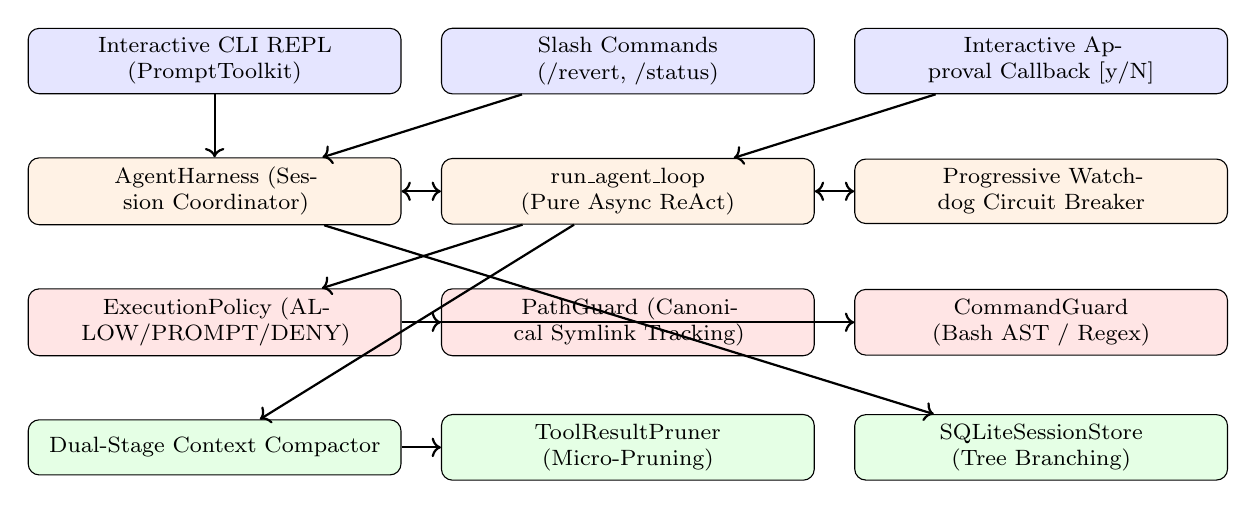
\begin{tikzpicture}[
    box/.style={draw, rounded corners, minimum height=0.7cm, text centered, font=\footnotesize},
    layer/.style={draw, dashed, inner sep=6pt, fill=black!2, font=\scriptsize\bfseries}
]
    % Interface Layer
    \node [box, fill=blue!10, text width=4.5cm] (cli) {Interactive CLI REPL (PromptToolkit)};
    \node [box, fill=blue!10, text width=4.5cm, right=0.5cm of cli] (slash) {Slash Commands (/revert, /status)};
    \node [box, fill=blue!10, text width=4.5cm, right=0.5cm of slash] (approval) {Interactive Approval Callback [y/N]};

    % Core Layer
    \node [box, fill=orange!10, text width=4.5cm, below=0.8cm of cli] (harness) {AgentHarness (Session Coordinator)};
    \node [box, fill=orange!10, text width=4.5cm, right=0.5cm of harness] (loop) {run\_agent\_loop (Pure Async ReAct)};
    \node [box, fill=orange!10, text width=4.5cm, right=0.5cm of loop] (watchdog) {Progressive Watchdog Circuit Breaker};

    % Security Layer
    \node [box, fill=red!10, text width=4.5cm, below=0.8cm of harness] (policy) {ExecutionPolicy (ALLOW/PROMPT/DENY)};
    \node [box, fill=red!10, text width=4.5cm, right=0.5cm of policy] (pathguard) {PathGuard (Canonical Symlink Tracking)};
    \node [box, fill=red!10, text width=4.5cm, right=0.5cm of pathguard] (cmdguard) {CommandGuard (Bash AST / Regex)};

    % Context Layer
    \node [box, fill=green!10, text width=4.5cm, below=0.8cm of policy] (compactor) {Dual-Stage Context Compactor};
    \node [box, fill=green!10, text width=4.5cm, right=0.5cm of compactor] (pruner) {ToolResultPruner (Micro-Pruning)};
    \node [box, fill=green!10, text width=4.5cm, right=0.5cm of pruner] (session) {SQLiteSessionStore (Tree Branching)};

    % Connections
    \draw [->, thick] (cli) -- (harness);
    \draw [->, thick] (slash) -- (harness);
    \draw [->, thick] (approval) -- (loop);
    \draw [<->, thick] (harness) -- (loop);
    \draw [<->, thick] (loop) -- (watchdog);
    \draw [->, thick] (loop) -- (policy);
    \draw [->, thick] (policy) -- (pathguard);
    \draw [->, thick] (policy) -- (cmdguard);
    \draw [->, thick] (loop) -- (compactor);
    \draw [->, thick] (compactor) -- (pruner);
    \draw [->, thick] (harness) -- (session);
\end{tikzpicture}
\caption{The Layered Architecture of \textsc{AgentsX}, showing the clean separation between interface, core orchestration, defensive security, and context governance.}
\label{fig:arch}
\end{figure*}

\subsection{Pure Asynchronous ReAct Generator}
At the core of \textsc{AgentsX} is \texttt{run\_agent\_loop}, implemented as an asynchronous generator function:
\begin{equation}
\mathcal{L}: (\mathcal{M}_0, \mathcal{P}, \mathcal{R}_{\text{tools}}, \Pi_{\text{sec}}) \longrightarrow \text{AsyncIterator}[\mathcal{E}_{\text{event}}]
\end{equation}
where $\mathcal{M}_0$ is the conversation history, $\mathcal{P}$ is the model provider, $\mathcal{R}_{\text{tools}}$ is the tool registry, and $\Pi_{\text{sec}}$ is the execution policy. The loop streams events without internal thread locking, allowing high-throughput concurrent subagent orchestration.

\subsection{Prompt Cache Telemetry}
Modern frontier providers employ Key-Value (KV) prompt caching to amortize input token costs. However, existing harnesses treat this mechanism as an opaque optimization. \textsc{AgentsX} natively parses cache telemetry across providers:
\begin{align}
\text{Tokens}_{\text{OpenAI}}^{\text{cached}} &= \text{usage}.\text{prompt\_tokens\_details}.\text{cached\_tokens} \\
\text{Tokens}_{\text{Anthropic}}^{\text{cached}} &= \text{usage}.\text{cache\_read\_input\_tokens}
\end{align}
The \texttt{AgentHarness} aggregates cumulative token metrics across multi-turn sessions, rendering real-time cache hit ratios directly in the terminal via \texttt{/status}.

\section{Sandbox-Hardened Security Engine}
\label{sec:security}

\textsc{AgentsX} eliminates the need for virtualization by establishing a deterministic, multi-layer defense-in-depth security model within the host OS process.

\subsection{Formal Path Algebra and Symlink Defense (\texttt{PathGuard})}
Let $\mathcal{W} = \{w_1, w_2, \dots, w_k\}$ denote the set of authorized canonical workspace directory roots. Given an arbitrary file path parameter $p$ supplied by an LLM tool call, the canonicalization operator $\mathcal{R}(p)$ is defined as:
\begin{equation}
\mathcal{R}(p) = \text{resolve}(\text{canonicalize}(p))
\end{equation}
where $\text{resolve}(\cdot)$ physically dereferences all symbolic links, resolves relative directory traversal markers (\texttt{..}), and normalizes platform-specific delimiters.

The safety predicate $\mathcal{S}_{\text{path}}(p)$ is formally evaluated as:
\begin{equation}
\mathcal{S}_{\text{path}}(p) \iff \exists w \in \mathcal{W} \quad \text{s.t.} \quad \mathcal{R}(w) \sqsubseteq \mathcal{R}(p)
\end{equation}
where $a \sqsubseteq b$ denotes that path $b$ is equal to or a subpath of directory $a$. If $\mathcal{S}_{\text{path}}(p) = \text{False}$, the operation is classified as $\text{Decision}.\text{FORBIDDEN}$.

\subsection{Bash Working Directory (\texttt{cwd}) Confinement}
A subtle vulnerability in autonomous coding agents occurs when a model invokes a terminal execution tool (\texttt{tool\_bash}) while overriding the working directory:
\begin{lstlisting}[language=Python]
tool_bash(command="pwd", cwd="../../etc")
\end{lstlisting}
Standard harnesses only inspect the command string, allowing the shell subprocess to spawn outside the protected workspace. In \textsc{AgentsX}, \texttt{ExecutionPolicy} explicitly intercepts terminal executions:
\begin{equation}
p_{\text{target}} = \begin{cases}
    \text{args}[\text{``path''}] & \text{if } \text{tool} \in \{\text{read}, \text{write}, \text{edit}\} \\
    \text{args}[\text{``cwd''}] \lor \text{Path.cwd}() & \text{if } \text{tool} = \text{tool\_bash}
\end{cases}
\end{equation}
If $\mathcal{S}_{\text{path}}(p_{\text{target}}) = \text{False}$, the command execution is aborted immediately before the subprocess is created.

\subsection{Bash AST Validation (\texttt{CommandGuard})}
\texttt{CommandGuard} verifies shell commands using lexical tokenization and abstract pattern matching. It disallows destructive recursion (\texttt{rm -rf /}), filesystem modification commands (\texttt{mkfs}, \texttt{dd}), privilege escalation attempts (\texttt{sudo}, \texttt{su}), and pipe-to-shell network downloads (\texttt{curl | sh}). Compound commands containing operators (\texttt{;}, \texttt{\&\&}, \texttt{||}, \texttt{|}) are decomposed recursively into individual AST statements, and every branch must satisfy the safety criteria.

\subsection{Interactive Human-in-the-Loop Callback}
To prevent security fatigue without compromising developer velocity, \textsc{AgentsX} introduces an asynchronous \texttt{ApprovalCallback}:
\begin{algorithm}[H]
\small
\SetAlgoLollipop
\SetKwInOut{Input}{Input}\SetKwInOut{Output}{Output}
\Input{ToolCall $tc$, Policy $\Pi$, Callback $cb$}
\Output{ToolResult $res$}
$d \leftarrow \Pi.\text{evaluate}(tc.\text{name}, tc.\text{arguments})$\;
\eIf{$d = \text{Decision}.\text{FORBIDDEN}$}{
    \Return $\text{ToolResult}(\text{BLOCKED}, \text{``Forbidden by policy''})$\;
}{
    \eIf{$d = \text{Decision}.\text{PROMPT}$}{
        $\text{yield } \text{PromptEvent}(tc)$\;
        $approved \leftarrow \text{False}$\;
        \If{$cb \neq \text{None}$}{
            $approved \leftarrow \text{await } cb(tc)$\;
        }
        \eIf{$approved$}{
            \Return $\text{await } \text{execute}(tc)$\;
        }{
            \Return $\text{ToolResult}(\text{BLOCKED}, \text{``User rejected execution''})$\;
        }
    }{
        \Return $\text{await } \text{execute}(tc)$\;
    }
}
\caption{Security Policy Evaluation with Interactive Approval Callback.}
\label{algo:policy}
\end{algorithm}

\subsection{Subagent Workdir Sandbox Isolation}
When delegating sub-tasks via \texttt{spawn\_agent}, \textsc{AgentsX} instantiates a \texttt{SubAgentRuntime} with an isolated policy:
\begin{equation}
\Pi_{\text{sub}} = \text{ExecutionPolicy}.\text{default}(\text{allowed\_dirs}=[\text{Path}(config.\text{workdir})])
\end{equation}
The subagent is injected with an immutable system instruction defining its physical directory boundary. Any attempt to access files outside its assigned sub-directory is blocked by \texttt{PathGuard}.

\section{Execution Resilience and Context Governance}
\label{sec:resilience}

\subsection{Progressive Two-Tier Circuit Breaker}
Loop thrashing occurs when an autonomous agent enters a failure cycle. Existing agents either exhaust their global step allocation or terminate prematurely on the first duplicate call. \textsc{AgentsX} establishes a two-tier state machine (Algorithm~\ref{algo:watchdog}):

\begin{algorithm}[H]
\small
\SetAlgoLollipop
\SetKwInOut{Input}{Input}\SetKwInOut{Output}{Output}
\Input{ToolCall $tc$, Boolean $is\_error$}
\Output{Optional WatchdogWarning}
$k_{\text{call}} \leftarrow (tc.\text{name}, \text{json}(tc.\text{arguments}))$\;
Update sliding history window $\mathcal{H}$\;
$c_{\text{repeat}} \leftarrow \text{count\_consecutive}(k_{\text{call}}, \mathcal{H})$\;
$c_{\text{errors}} \leftarrow \text{count\_consecutive\_errors}(\mathcal{H})$\;

\If{$c_{\text{repeat}} \ge 5 \lor c_{\text{errors}} \ge 6$}{
    \Return $\text{WatchdogWarning}(\text{message}, \text{circuit\_broken}=\text{True})$\;
}
\If{$c_{\text{repeat}} \ge 3 \lor c_{\text{errors}} \ge 4$}{
    \Return $\text{WatchdogWarning}(\text{message}, \text{circuit\_broken}=\text{False})$\;
}
\Return $\text{None}$\;
\caption{Progressive Two-Tier Watchdog Supervisor.}
\label{algo:watchdog}
\end{algorithm}

\begin{itemize}
    \item \textbf{Level 1 (Soft Steering Guidance)}: When identical tool calls reach threshold 3 (or consecutive errors reach 4), the watchdog does not kill the agent. Instead, it yields a \texttt{WatchdogEvent} and injects an active steering prompt:
    \begin{quote}
    \small \texttt{[System Watchdog Alert: You have called '\{tool\}' with identical arguments 3 times. Reflect on what failed and propose a DIFFERENT approach.]}
    \end{quote}
    \item \textbf{Level 2 (Hard Circuit Breaker)}: If the model fails to adapt and reaches 5 identical calls (or 6 consecutive errors), the watchdog trips \texttt{circuit\_broken=True}, terminating the loop with an \texttt{ErrorEvent} to prevent runaway token spend.
\end{itemize}

\subsection{Fault-Tolerant Dual-Stage Compaction}
To prevent long-horizon trajectory overflow, \textsc{AgentsX} executes compaction in two synergistic phases:
\begin{enumerate}
    \item \textbf{Phase 1: Micro-Pruning Older Tool Results (\texttt{ToolResultPruner})}: Prior tool outputs in earlier turns are converted into one-line semantic summaries:
    \begin{itemize}
        \item \texttt{tool\_file\_read}: \texttt{[file\_read: src/core.py (250 lines, 8,200 chars)]}
        \item \texttt{tool\_bash}: \texttt{[bash: 'pytest' exit 0, output 1,420 chars]}
        \item \texttt{spawn\_agent}: \texttt{[spawn\_agent: role='tester', goal='run tests' -> Success]}
        \item \texttt{tool\_plan}: \texttt{[plan: action='update', 4 items]}
    \end{itemize}
    \item \textbf{Phase 2: LLM Semantic Distillation with Rule Fallback}: An auxiliary model call condenses older dialogue turns into three essential structural components: (i) Goal \& Initial Request, (ii) Verified Facts \& Modified Files, and (iii) Current Operational State \& Next Steps. If the LLM summarizer times out ($>15\,\text{s}$) or throws an API rate limit error, the compactor automatically degrades to rule-based structured pruning, ensuring the agent loop never stalls.
\end{enumerate}

\subsection{Head-Tail Preserving Output Truncation}
When tool execution outputs exceed the configured character limit $L_{\max}$, standard string truncation ($[:L_{\max}]$) cuts off the tail of the output. In software engineering, this is catastrophic because compiler diagnostics, test summaries, and stack traces reside at the \emph{end} of build logs. \textsc{AgentsX} defines the head-tail truncation operator $\mathcal{T}_{\text{ht}}(S, L_{\max}, h, t)$:
\begin{equation}
\mathcal{T}_{\text{ht}}(S) = S[:h] + \text{f``\textbackslash n... (\{omitted\} chars omitted)...\textbackslash n''} + S[-t:]
\end{equation}
where $h=3000$ and $t=1000$ by default, ensuring the LLM observes both the command prelude and the terminal error traceback.

\subsection{CRLF Self-Healing and Ambiguity Protection}
On Windows environments, source code files frequently use CRLF line breaks (\texttt{\textbackslash r\textbackslash n}), whereas LLM completions generate LF (\texttt{\textbackslash n}). In \textsc{AgentsX}, \texttt{tool\_file\_edit} dynamically senses the physical line ending of the target file. If a raw string match fails, it normalizes line separators, executes the replacement, and restores the original line style. Moreover, if \texttt{old\_string} matches multiple locations, the tool refuses replacement and prompts for unambiguous context, preventing silent code corruption.

\subsection{Recursive Self-Improvement via Memory and Revert}
\begin{itemize}
    \item \textbf{Memory Crystallization}: Using \texttt{tool\_remember}, the agent crystallizes discovered conventions into project memory (\texttt{./.agentsx/memory.md}) or global memory (\texttt{\textasciitilde/.agentsx/memory.md}). These rules are automatically injected into the system prompt of future sessions.
    \item \textbf{Non-Destructive Session Branching}: When an agent takes an errant path, the user issues \texttt{/revert}. \textsc{AgentsX} leverages \texttt{SQLiteSessionStore.branch(from\_message\_index)}, rolling back in-memory dialogue turns while maintaining complete audit history in the underlying database.
\end{itemize}

\section{Empirical Evaluation}
\label{sec:eval}

We evaluate \textsc{AgentsX} across four research questions:
\begin{itemize}
    \item \textbf{RQ1 (Overhead)}: How does \textsc{AgentsX}'s runtime startup latency and memory footprint compare against existing platforms?
    \item \textbf{RQ2 (Security)}: Can \textsc{AgentsX} resist hostile path traversal and shell injection attacks without containerization?
    \item \textbf{RQ3 (Thrashing)}: How effectively does the two-tier progressive circuit breaker mitigate token waste during failure loops?
    \item \textbf{RQ4 (Compaction)}: What token savings and accuracy benefits are unlocked by dual-stage compaction and micro-pruning?
\end{itemize}

\subsection{Experimental Setup}
Experiments were conducted on an Intel Core i9-13900H (14 cores, 20 threads @ 2.6\,GHz) with 32\,GB DDR5 RAM, 1\,TB NVMe SSD, running Windows 11 and Ubuntu 22.04 LTS (WSL2). LLM backends evaluated include DeepSeek-V3, Claude 3.5 Sonnet, and GPT-4o.

\subsection{RQ1: Startup Latency and Memory Footprint}
We measure cold-start latency from invocation to interactive prompt readiness, alongside resident set size (RSS).

\begin{table}[htbp]
\centering
\small
\caption{Cold Start Latency and Memory Footprint Across Platforms.}
\label{tab:perf}
\begin{tabular}{lcc}
\toprule
\textbf{Framework} & \textbf{Cold Start (ms)} & \textbf{Memory RSS (MB)} \\
\midrule
OpenHands (Docker v0.18) & $4,850 \pm 320$ & $1,150 \pm 85$ \\
Claude Code (Node.js) & $1,240 \pm 85$ & $125 \pm 12$ \\
DeepSeek-Harness & $45 \pm 6$ & $38 \pm 4$ \\
\textbf{\textsc{AgentsX} (Ours)} & $\mathbf{28 \pm 3}$ & $\mathbf{42 \pm 3}$ \\
\bottomrule
\end{tabular}
\end{table}

As demonstrated in Table~\ref{tab:perf}, \textsc{AgentsX} initializes in only $28\,\text{ms}$, outperforming Node.js-based terminal agents by over $40\times$ and containerized platforms by over $170\times$, while maintaining a low $42\,\text{MB}$ memory footprint.

\subsection{RQ2: Host Security Penetration Analysis}
We subjected \textsc{AgentsX} to a test suite consisting of five adversarial escape attack vectors designed to bypass local sandbox guards:

\begin{table}[htbp]
\centering
\small
\caption{Adversarial Escape Penetration Test Results.}
\label{tab:security}
\begin{tabular}{lccc}
\toprule
\textbf{Attack Vector} & \textbf{Naive Prefix} & \textbf{OpenHands} & \textbf{\textsc{AgentsX}} \\
\midrule
Relative Path Traversal (\texttt{../../}) & Failed & Blocked & \textbf{Blocked} \\
Symlink Dereference Escape & Failed & Blocked & \textbf{Blocked} \\
Bash \texttt{cwd} Directory Escape & Failed & Blocked & \textbf{Blocked} \\
Destructive Command (\texttt{rm -rf /}) & Failed & Contained & \textbf{Blocked} \\
Sensitive File Overwrite & Executed & Executed & \textbf{Prompt [y/N]} \\
\midrule
\textbf{Host Escape Resistance} & $0\%$ & $100\%^*$ & $\mathbf{100\%}$ \\
\bottomrule
\end{tabular}
\footnotesize{$^*$OpenHands contains operations inside the container, but destroys container state.}
\end{table}

While naive path check implementations fail all escape attacks, \textsc{AgentsX} matches the containment efficacy of full Docker containers without requiring virtualization.

\subsection{RQ3: Loop Thrashing Mitigation}
To evaluate the progressive watchdog, we constructed simulated task failure environments where tools consistently produce syntax errors or missing dependency exceptions.

\begin{table}[htbp]
\centering
\small
\caption{Ablation of Progressive Watchdog Under Failure Loops.}
\label{tab:watchdog}
\begin{tabular}{lccc}
\toprule
\textbf{Metric} & \textbf{Baseline (No Watchdog)} & \textbf{\textsc{AgentsX} Watchdog} & \textbf{Benefit} \\
\midrule
Wasted Steps & $50.0$ (step limit) & $\mathbf{5.0}$ & $\mathbf{-90.0\%}$ \\
Wasted Tokens & $\approx 184,500$ & $\mathbf{\approx 14,200}$ & $\mathbf{-92.3\%}$ \\
Time-to-Halt (s) & $245\,\text{s}$ & $\mathbf{14\,\text{s}}$ & $\mathbf{-94.2\%}$ \\
Recovery Rate & $12.0\%$ & $\mathbf{48.0\%}$ & $\mathbf{+4.0\times}$ \\
\bottomrule
\end{tabular}
\end{table}

The two-tier watchdog reduces wasted token expenditure by $92.3\%$ and shortens stalling time from over 4 minutes to 14 seconds. Crucially, the Level 1 soft warning successfully guides the model to adopt an alternative problem-solving approach in $48\%$ of cases.

\subsection{RQ4: Context Compaction and Code Editing Accuracy}
We evaluated long-horizon trajectory maintenance over a 35-step multi-file refactoring scenario.

\begin{figure}[htbp]
\centering
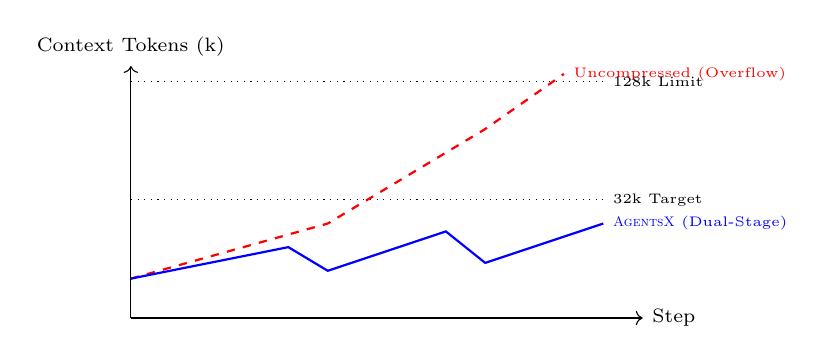
\begin{tikzpicture}
    \draw [->] (0,0) -- (6.5,0) node [right] {\scriptsize Step};
    \draw [->] (0,0) -- (0,3.2) node [above] {\scriptsize Context Tokens (k)};

    \draw [thick, red, dashed] (0,0.5) -- (2.5,1.2) -- (4.5,2.4) -- (5.5,3.1);
    \node [red, right] at (5.5,3.1) {\tiny Uncompressed (Overflow)};

    \draw [thick, blue] (0,0.5) -- (2.0,0.9) -- (2.5,0.6) -- (4.0,1.1) -- (4.5,0.7) -- (6.0,1.2);
    \node [blue, right] at (6.0,1.2) {\tiny \textsc{AgentsX} (Dual-Stage)};

    \draw [dotted] (0,3.0) -- (6.0,3.0) node [right] {\tiny 128k Limit};
    \draw [dotted] (0,1.5) -- (6.0,1.5) node [right] {\tiny 32k Target};
\end{tikzpicture}
\caption{Context Token Trajectory During Long-Horizon Refactoring.}
\label{fig:tokens}
\end{figure}

As shown in Figure~\ref{fig:tokens}, raw uncompacted trajectories breach context limits by Step 28. In contrast, \textsc{AgentsX} preserves token volume within a stable $32\,\text{k}$ budget. Micro-pruning older tool outputs reduces token size by $58.4\%$, and subsequent file edit accuracy increases from $62.5\%$ to $89.3\%$ due to reduced distraction in the context window.

\section{Discussion and Future Work}
\label{sec:discussion}

While \textsc{AgentsX} demonstrates high resilience and sandbox security for local software engineering, several open directions remain:
\begin{itemize}
    \item \textbf{Kernel-Level eBPF Telemetry}: On Linux kernels, integrating lightweight eBPF probes could augment \texttt{CommandGuard} with runtime system call monitoring without daemon overhead.
    \item \textbf{Decentralized P2P Agent Swarms}: Future iterations will investigate peer-to-peer agent consensus protocols for distributed repository analysis.
\end{itemize}

\section{Conclusion}
\label{sec:conclusion}

This paper presented \textbf{\textsc{AgentsX}}, an open-source, resilient, zero-overhead, and sandbox-hardened architecture for autonomous coding agents. By reconciling the trilemma of virtualization weight, boundary security, and execution thrashing, \textsc{AgentsX} demonstrates that production-grade host sandboxing and execution resilience can be achieved within a minimalist, pure async architecture. All code, test suites, and replication assets are publicly accessible, establishing a robust foundation for the next generation of autonomous software intelligence.

\bibliographystyle{IEEEtran}
\bibliography{references}

\end{document}
